\subsection{Simulation of maximal parallel P system} % (fold)
\label{sub:simulation_of_maximal_parallel_p_system}

The last lemmas (\ref{lemma:context_rules} and \ref{lemma:inhibitor_step}) will simplify the proof of the following theorem.

\begin{veta}
% TODO: rozdelit na viac liem
  The sequential P system with inhibitors defines the same Parikh image of language as P system with maximal parallelism.
\end{veta}

\begin{dokaz}
  We will prove the theorem by simulation.
  The proof is quite technical with some workarounds.
  For every computation of the maximal parallel P system $\Pi$ we will find a computation of the sequential P system with inhibitors $\overline{\Pi}$ with the same result.
  The computation to simulate is a sequence of maximal parallel steps.
  In each step of $\Pi$, a maximal multiset of rewriting rules are applied in each membrane.
  We simulate this maximal parallel step with several steps of sequential system $\overline{\Pi}$.

  We must prevent rule applying from the next maximal parallel step as that would be an incorrect simulation.
  Preventing this will be done with synchronization.
  Every membrane will have a state, represented as an object.
  The most important states are $RUN$ and $SYNCHRONIZE$.
  In the $RUN$ state, rewriting rules of $\Pi$ are applied until there is no rule to be appied. Then, the membrane proceeds to the $SYNCHRONIZE$ state.
  All the membranes in $SYNCHRONIZE$ step are waiting for other membranes to reach $SYNCHRONIZE$ step, so they all can proceed to the $RUN$ state of the next maximal parallel step of $\Pi$.

  Other states are just technical - we need to implement sending objects between membranes and preparing for the next maximal parallel step by clearing temporary objects.

  More detailed description of states:
  

  \begin{itemize}
    \item $RUN$: Rewriting occurs.
    To prevent double rewriting, we mark the products of rules with $a^{\prime}$ instead of $a$.
    Objects that are to be sent to the parent membrane are directly sent because the parent membrane is already in $RUN$ or $SYNCHRONIZE$ state, so the $a^{\prime}$ symbols that are sent don't break anything.
    
    But objects that are to be sent down, can't be sent immediately because child membranes can be in the $RESTORE$ state restoring symbols from the previous maximal parallel step. Current symbols could interfere with them and be rewritten twice in this step. Such objects are only marked as ``to be sent down'': $a^{\downarrow\prime}$.

    When $RUN$ phase ends (in the membrane $i$), the $SYNCTOKEN_i$ is sent upwards to notify the skin membrane that the membrane $i$ is ready to be synchronized.

    \item $SYNCHRONIZE$: Rewriting has ended and membrane is waiting to get signal $SYNCED$ from the skin membrane to continue to the next state.

    \item $SENDDOWN$: Signal was caught and now all descendant membranes are in $SYNCHRONIZE$ phase. So objects $a^{\downarrow\prime}$ can be sent down.

    \item $RESTORE$: All $a^{\prime}$ symbols are restored to $a$ and other temporary symbols are cleared, so the next step of rewriting can take place.
  \end{itemize}

  \begin{figure}
    \def\svgwidth{\textwidth}
    \input{possible_pairs_of_states_of_parent_and_child_membrane.pdf_tex}
    % 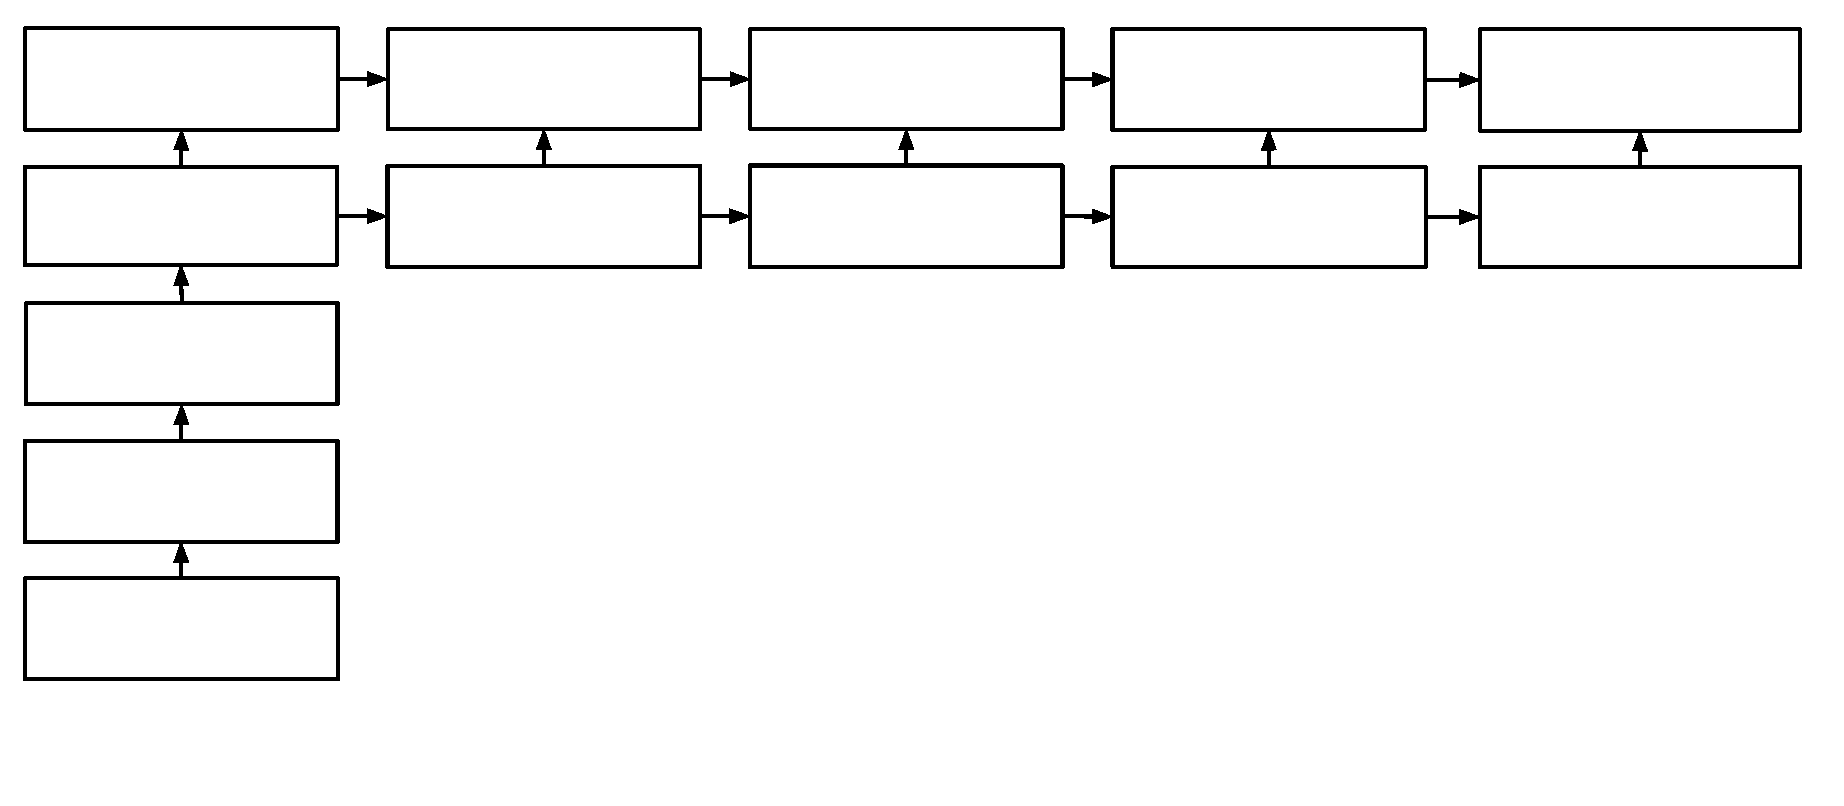
\includegraphics[width=\textwidth]{possible_pairs_of_states_of_parent_and_child_membrane}
    \caption{Possible pairs of states of parent and child membrane}
    \label{fig:possible_pairs_of_states_of_parent_and_child_membrane}
  \end{figure}

  In the figure \ref{fig:possible_pairs_of_states_of_parent_and_child_membrane} the pairs of states of parent and child membrane are joined with possible transitions between two consecutive global synchronizations - after the maximal parallel steps $i$ and $i+1$.
  

  % Rewriting rules

  \begin{itemize}
    \item For every rule $r_i\in R$ such that $r_i = a_1^{M(a_1)}a_2^{M(a_2)}\dots a_n^{M(a_n)} \rightarrow a_1^{N(a_1)}a_2^{N(a_2)}\dots a_n^{N(a_n)}$ we will have the following rules:
  
    $a_1^{M(a_1)-m_1}\dot{a}_1^{m_1}a_2^{M(a_2)-m_2}\dot{a}_2^{m_2}\dots a_n^{M(a_n)-m_n}\dot{a}_n^{m_n}|RUN \rightarrow a_1^{\prime N(a_1)}a_2^{\prime N(a_2)}\dots a_n^{\prime N(a_n)}|RUN$

    There will be such rule for each $0\leq m_i\leq M(a_i)$. It represents the idea that $\dot{a}$ can be used in rewriting in the same way as $a$. Right side of the rules contains symbols $a^\prime$, that prevents the symbols to be rewritten again.

    \item For every symbol $a\in V$ we will have the following rules:

    $a|RUN \rightarrow \dot{a}|RUN|_{\neg \dot{a}}$

    There will be max one occurrence of $\dot{a}$.

    \item For every rule $r_i\in R$ there will be a rule that detects if the rule $r_i$ is not usable. According to left side of the rule $r_i$, symbol $UNUSABLE_i$ will be created when there is not enough objects to fire the rule $r_i$. It means that left side of rule $r_i$ requires more instances of some object than are present in membrane.

    If the left side is of type:
    \begin{itemize}
      \item $a$: It is a context free rule. The rule can't be used if there is no occurrence of $a$ nor $\dot{a}$.

      $RUN \rightarrow UNUSABLE_i|RUN|_{\neg\{UNUSABLE_i, a, \dot{a}\}}$

      \item $ab$: It is a cooperative rule with two distinct objects on the left side. The rule can't be used if there is one of them missing.

      $RUN \rightarrow UNUSABLE_i|RUN|_{\neg\{UNUSABLE_i, a, \dot{a}\}}$

      $RUN \rightarrow UNUSABLE_i|RUN|_{\neg\{UNUSABLE_i, b, \dot{b}\}}$

      \item $a^2$: It is a cooperative rule with two same objects. The rule can't be used if there is at most one occurrence of the symbol. That happens if there is no occurrence of $a$. There can still be $\dot{a}$, but at most one occurrence.

      $RUN \rightarrow UNUSABLE_i|RUN|_{\neg\{UNUSABLE_i, a\}}$
    \end{itemize}

    

    \item For every membrane with label $i$ there will be rule:

    $UNUSABLE_1|UNUSABLE_2|\dots|UNUSABLE_m|RUN \rightarrow SYNCHRONIZE|SYNCTOKEN_i\uparrow$

    If no rule can be used, maximal parallel step in the region is completed so it goes to synchronization phase and sends a synchronization token to the parent membrane. The objects $UNUSABLE_i$ are not consumed in other rules, so by Lemma \ref{lemma:context_rules} this rule can be written with set of cooperative rules.

    \item For every membrane other than the skin membrane, there will be a rule:

    $SYNCHRONIZE|SYNCTOKEN_j \rightarrow SYNCHRONIZE|SYNCTOKEN_j\uparrow$

    Membrane resends all sync token to parent membrane.

    \item In skin membrane there is a rule which collects all the synchronization tokens from all membranes $1\dots k$ and then sends down signal that synchronization is complete. But before that, there can be some symbols that should be sent down, but they weren't, because the region below could have not started the rewriting phase that time. The result was just marked with $a^{\downarrow\prime}$.

    $SYNCTOKEN_1|SYNCTOKEN_2|\dots|SYNCTOKEN_k|SYNCHRONIZE \rightarrow SENDDOWN$

    The objects $SYNCTOKEN_i$ are not consumed in other rules in the skin membrane, so by Lemma \ref{lemma:context_rules} this rule can be written with set of cooperative rules.

    \item Every membrane other than skin membrane have to receive the signal to go to senddown phase:

    $SYNCHRONIZE|SYNCED \rightarrow SENDDOWN$

    \item Every membrane will have rules for every symbol $a\in V$ to send down all unsent object that should have been sent down:

    $SENDDOWN|a^{\downarrow\prime} \rightarrow SENDDOWN|a^{\prime}\downarrow$

    \item Every membrane will have rule for detecting when all such objects have been sent and it goes to restore phase:

    $SENDDOWN \rightarrow RESTORE|_{\neg \{a_i^{\downarrow\prime}|1\leq i\leq n\}}$

    \item In restore phase all symbols $a^{\prime}$ will be rewritten to $a$ in order to be able to be rewritten in next maximal parallel step:

    $RESTORE|a^{\prime} \rightarrow RESTORE|a$

    \item There may be some $GONE$ symbols left, which should be cleared too:

    $RESTORE|GONE_i \rightarrow RESTORE$

    \item When restore phase ends, it sends down signal that all membranes have been synchronized and next phase of rewriting has began in upper membranes:

    $RESTORE \rightarrow RUN|SYNCED\downarrow|_{\neg \{a_i^{\prime}|1\leq i\leq n\}\cup\{GONE_i|1\leq i\leq n\}}$
  \end{itemize}


  Phase of membrane is represented by object so the region is never empty and by the Lemma~\ref{lemma:inhibitor_step} the rules with set of inhibitors can be simulated by single inhibitors.
\end{dokaz}

% subsection simulation_of_maximal_parallel_p_system (end)